\subsection{Binary Tree}
\begin{frame}[fragile]
\frametitle{Binary Tree}
A {\bf binary tree} is a tree data structure in which each node has at most two children, which are referred to as the left child and the right child.\\
A {\bf binary \emph{search} tree} is a binary tree in which each internal node n stores an
element such that the element stored in the left subtree of n are less than n and
elements stored in the right subtree of n are greater than n.
\end{frame}

\begin{frame}[fragile]
\frametitle{Binary Search Tree - Insert}
Insert: 8, 3, 6, 10, 14, 4, 7, 1, 13\\
\vspace{3mm}
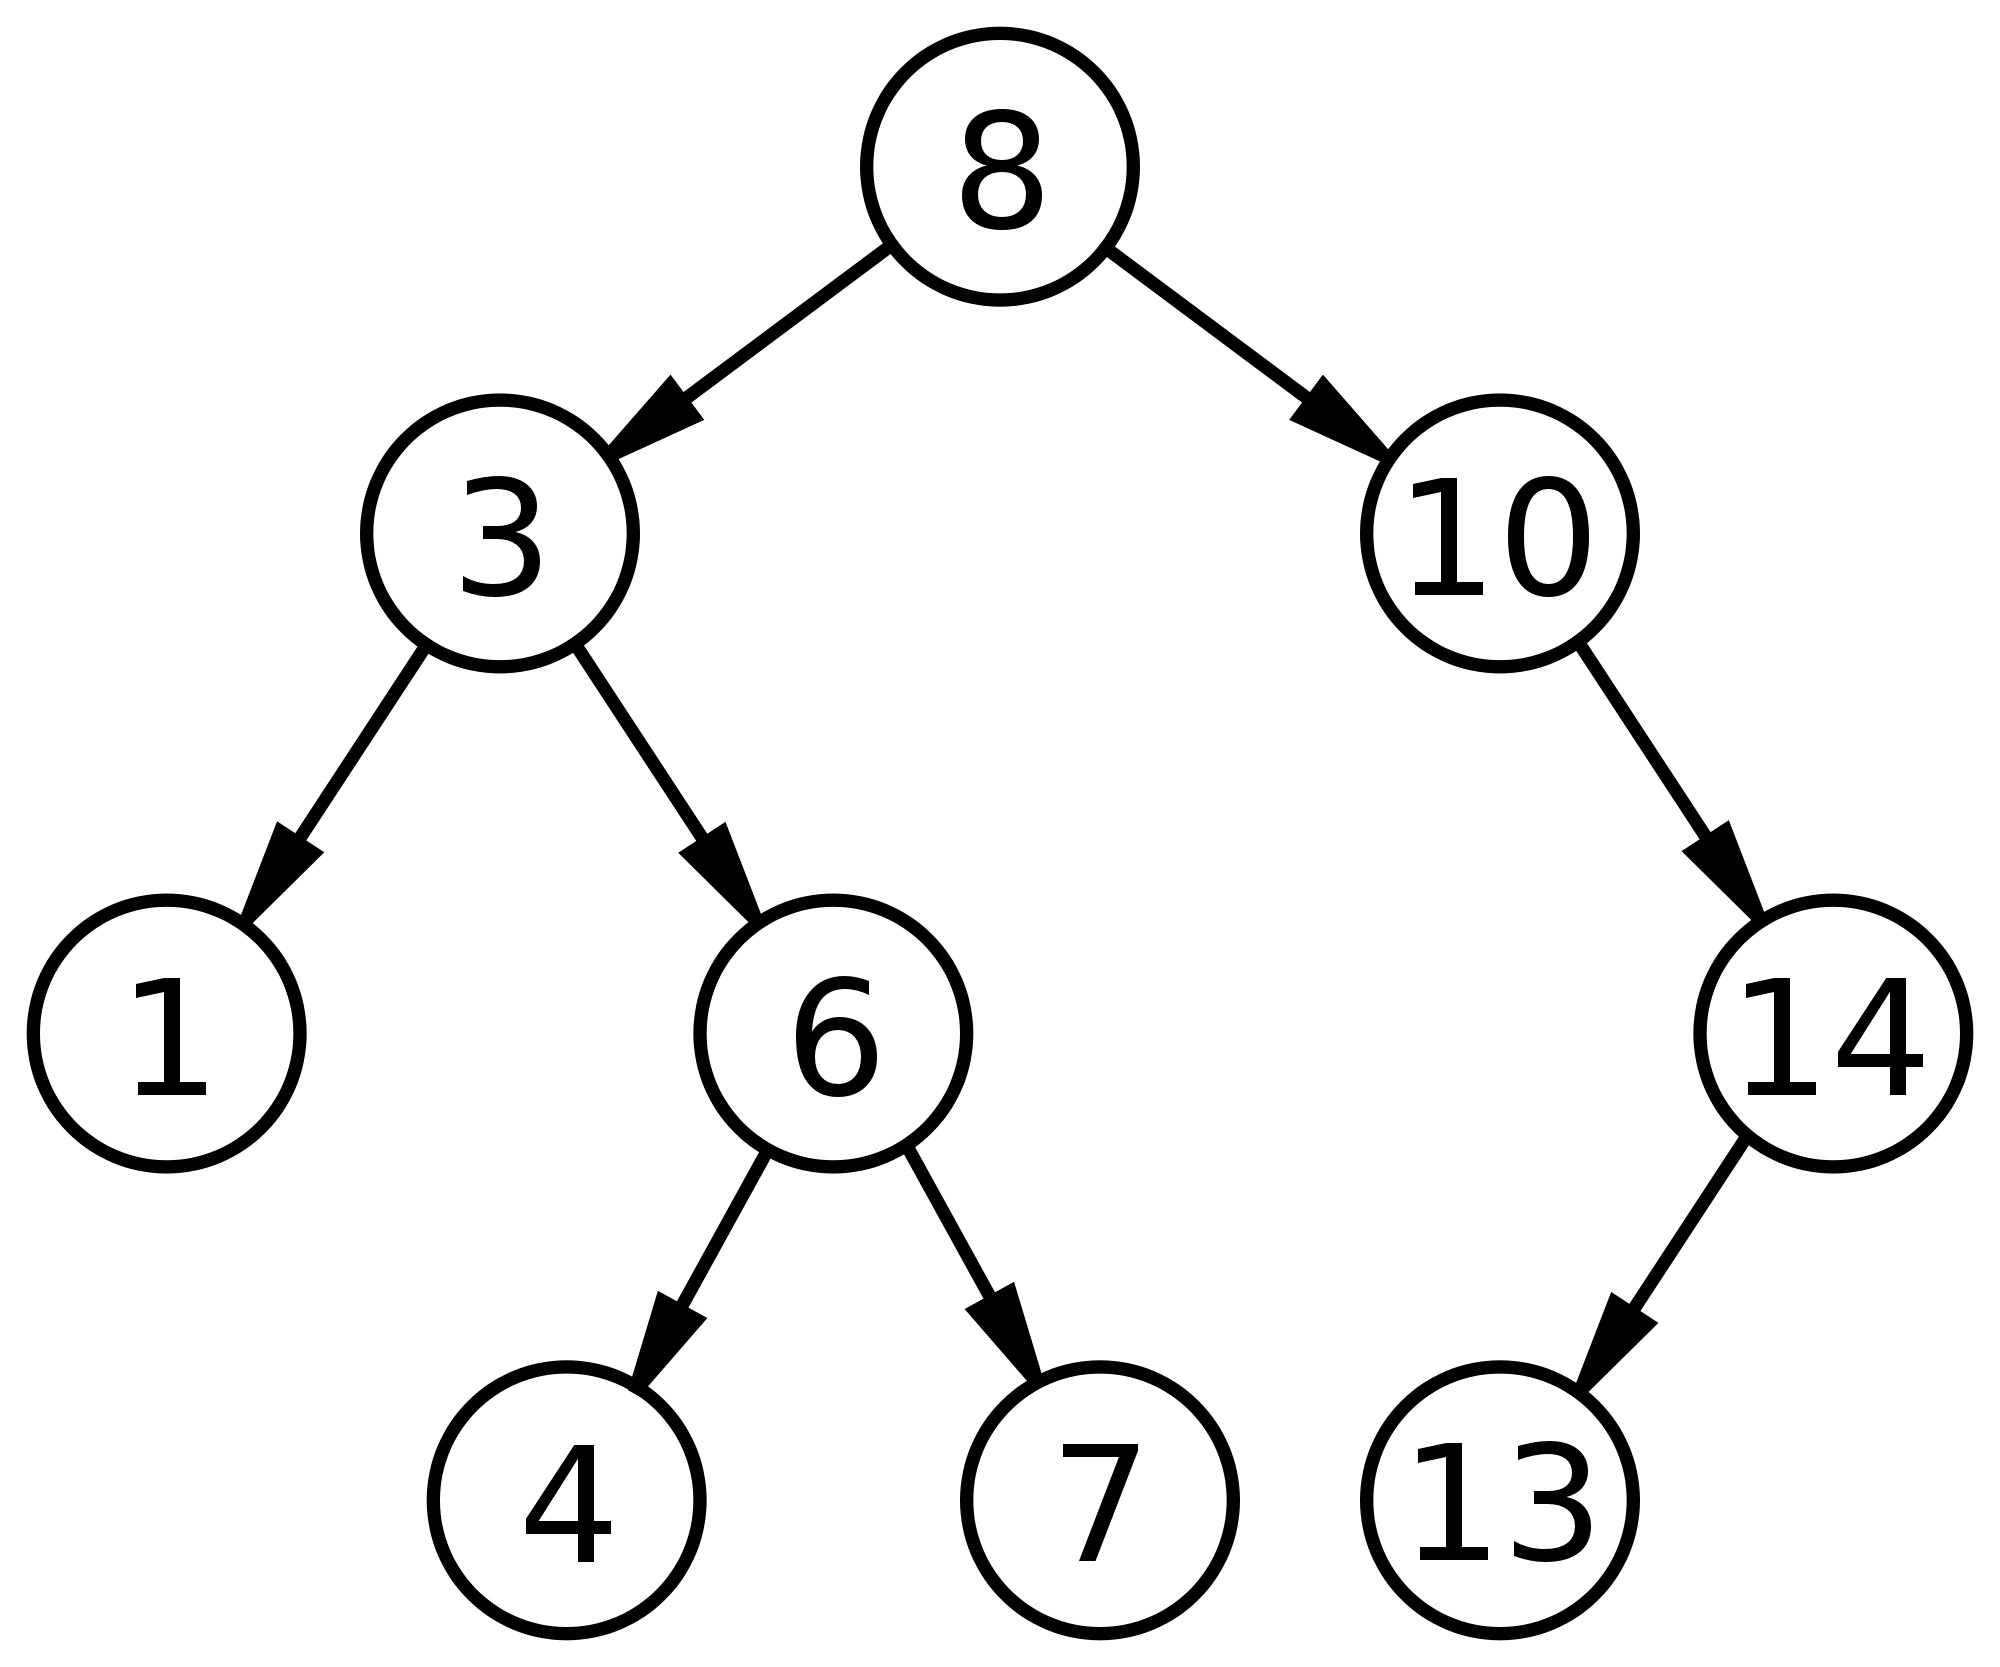
\includegraphics[scale=0.05]{img/binarytree_2.png}
\end{frame}

\begin{frame}[fragile]
\frametitle{Binary Search Tree - Delete Leaf Node}
Delete: 4\\
\vspace{3mm}
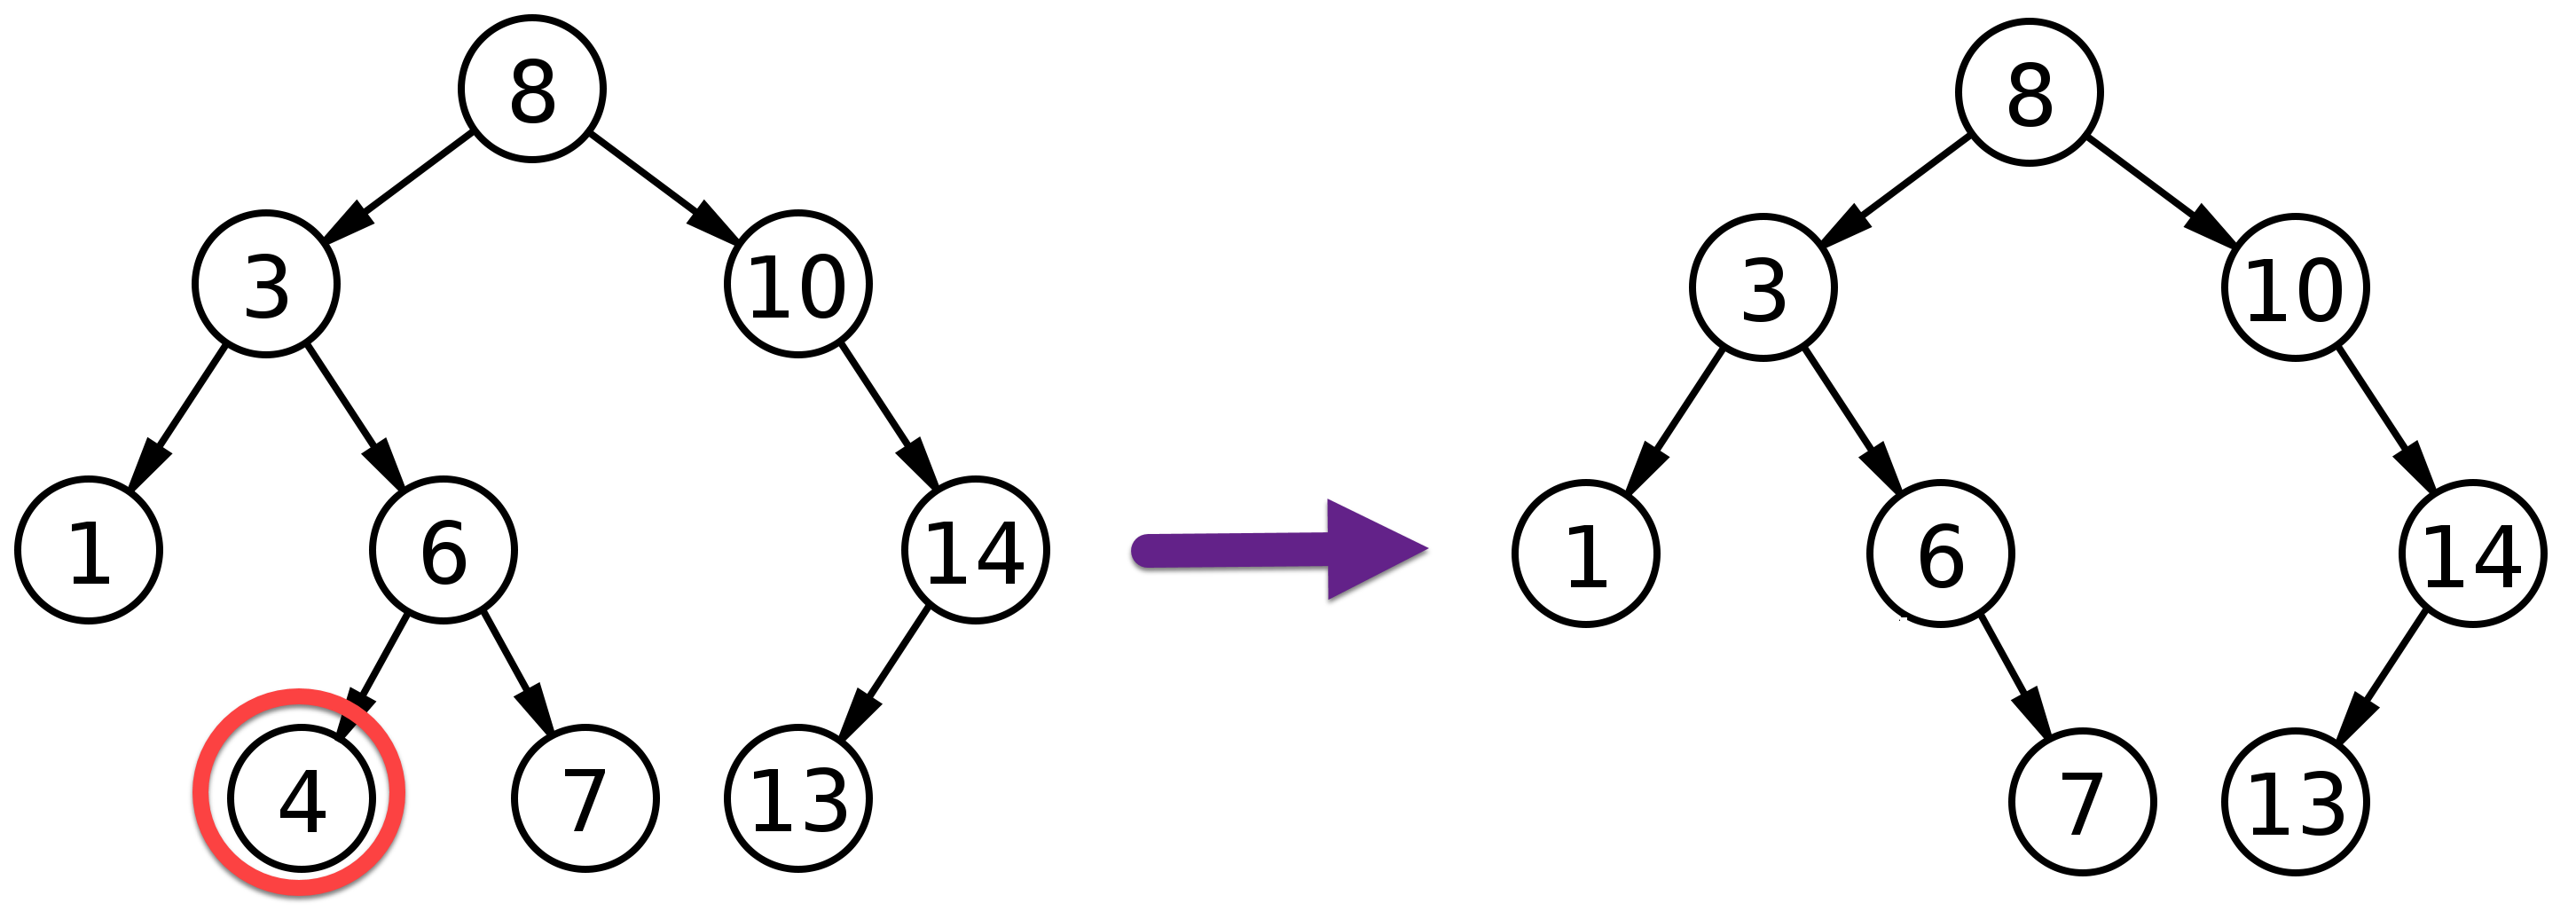
\includegraphics[scale=0.14]{img/tree2.png}
\end{frame}

\begin{frame}[fragile]
\frametitle{Binary Search Tree - Delete Node with 1 Successor}
Delete: 14\\
\vspace{3mm}
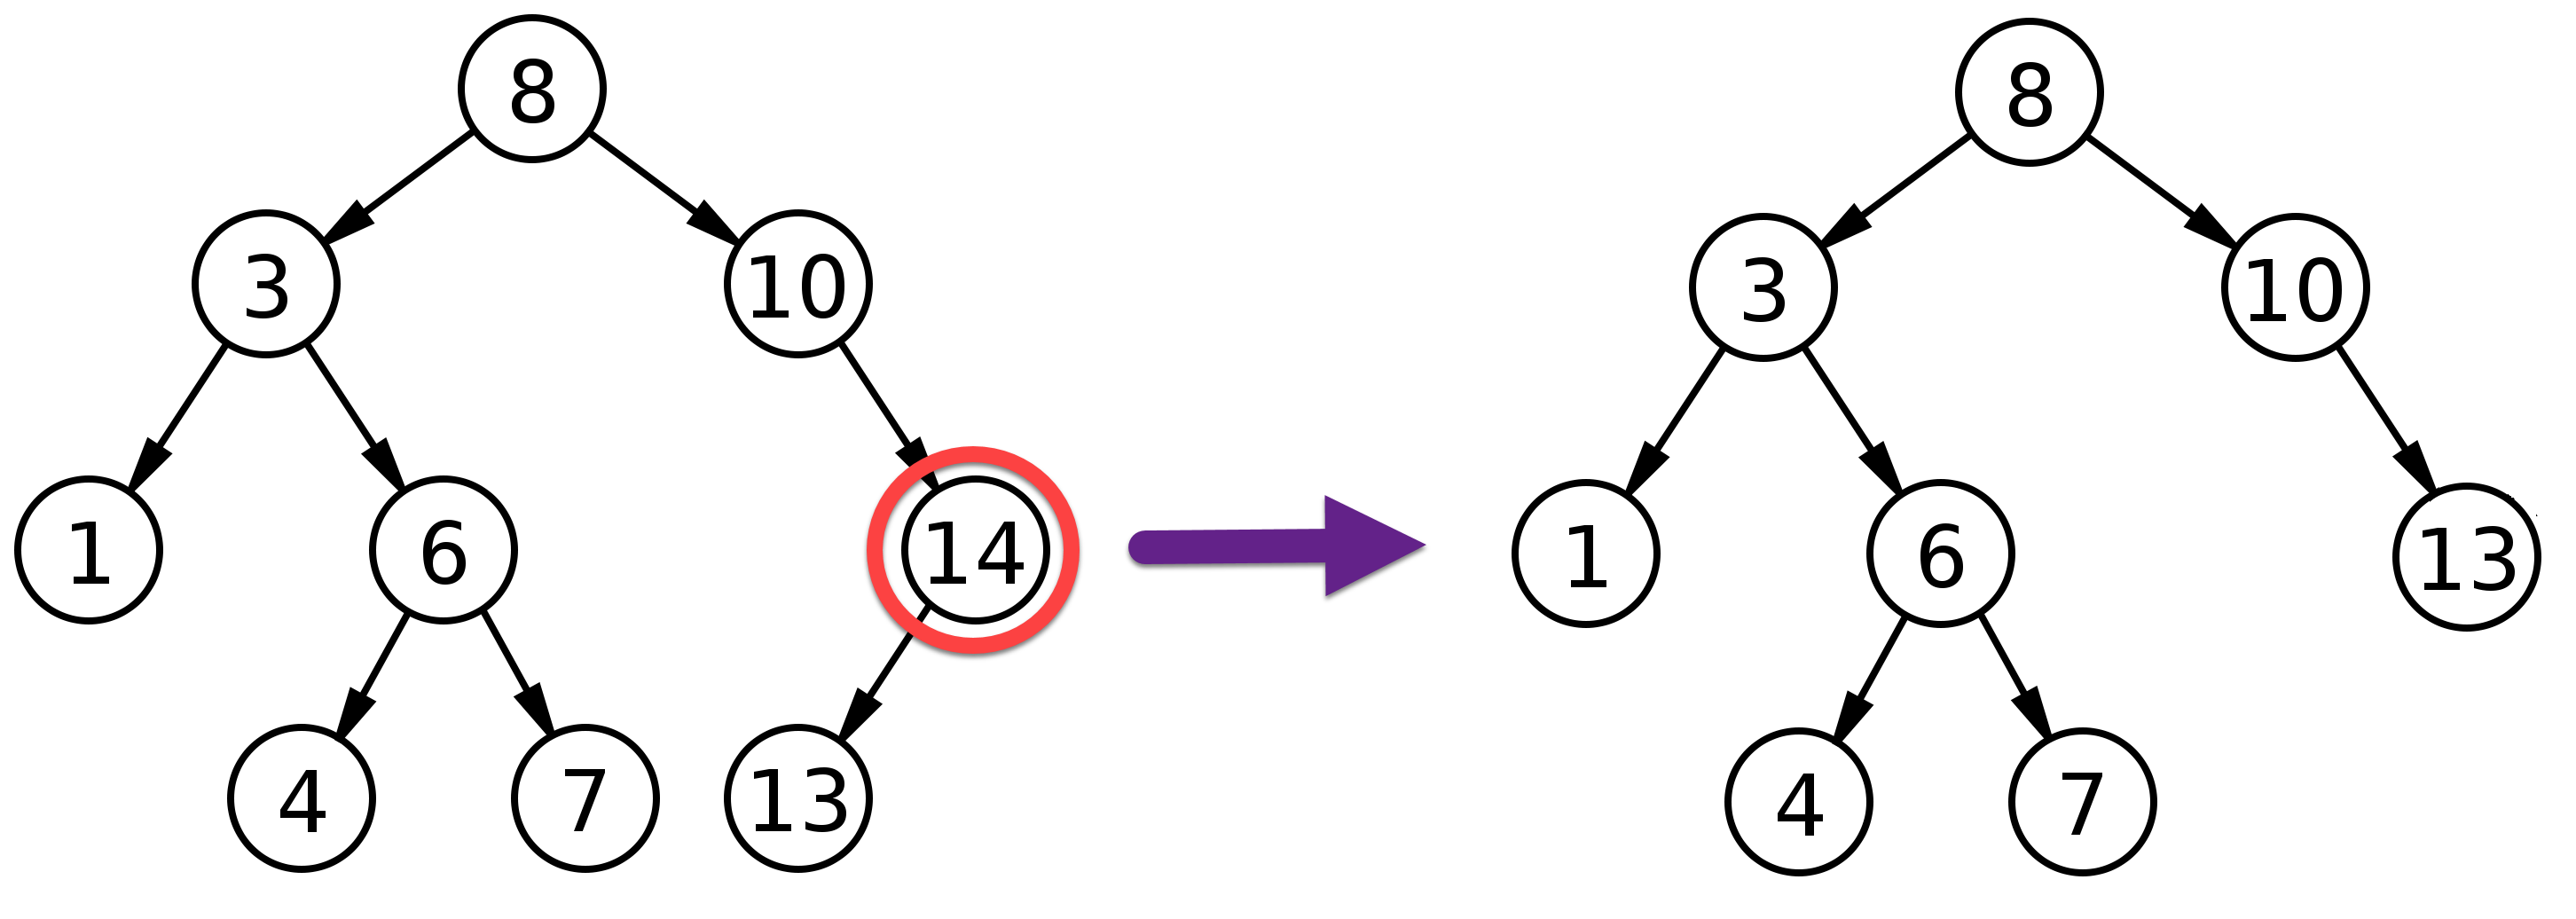
\includegraphics[scale=0.14]{img/tree3.png}
\end{frame}

\begin{frame}[fragile]
\frametitle{Binary Search Tree - Delete Node with 2 Succesors}
Delete: 3\\
Replace the node with one of the following two nodes:
\begin{itemize}
\item The most right node in the left sub tree
\item The most left node in the right sub tree
\end{itemize}
\vspace{3mm}
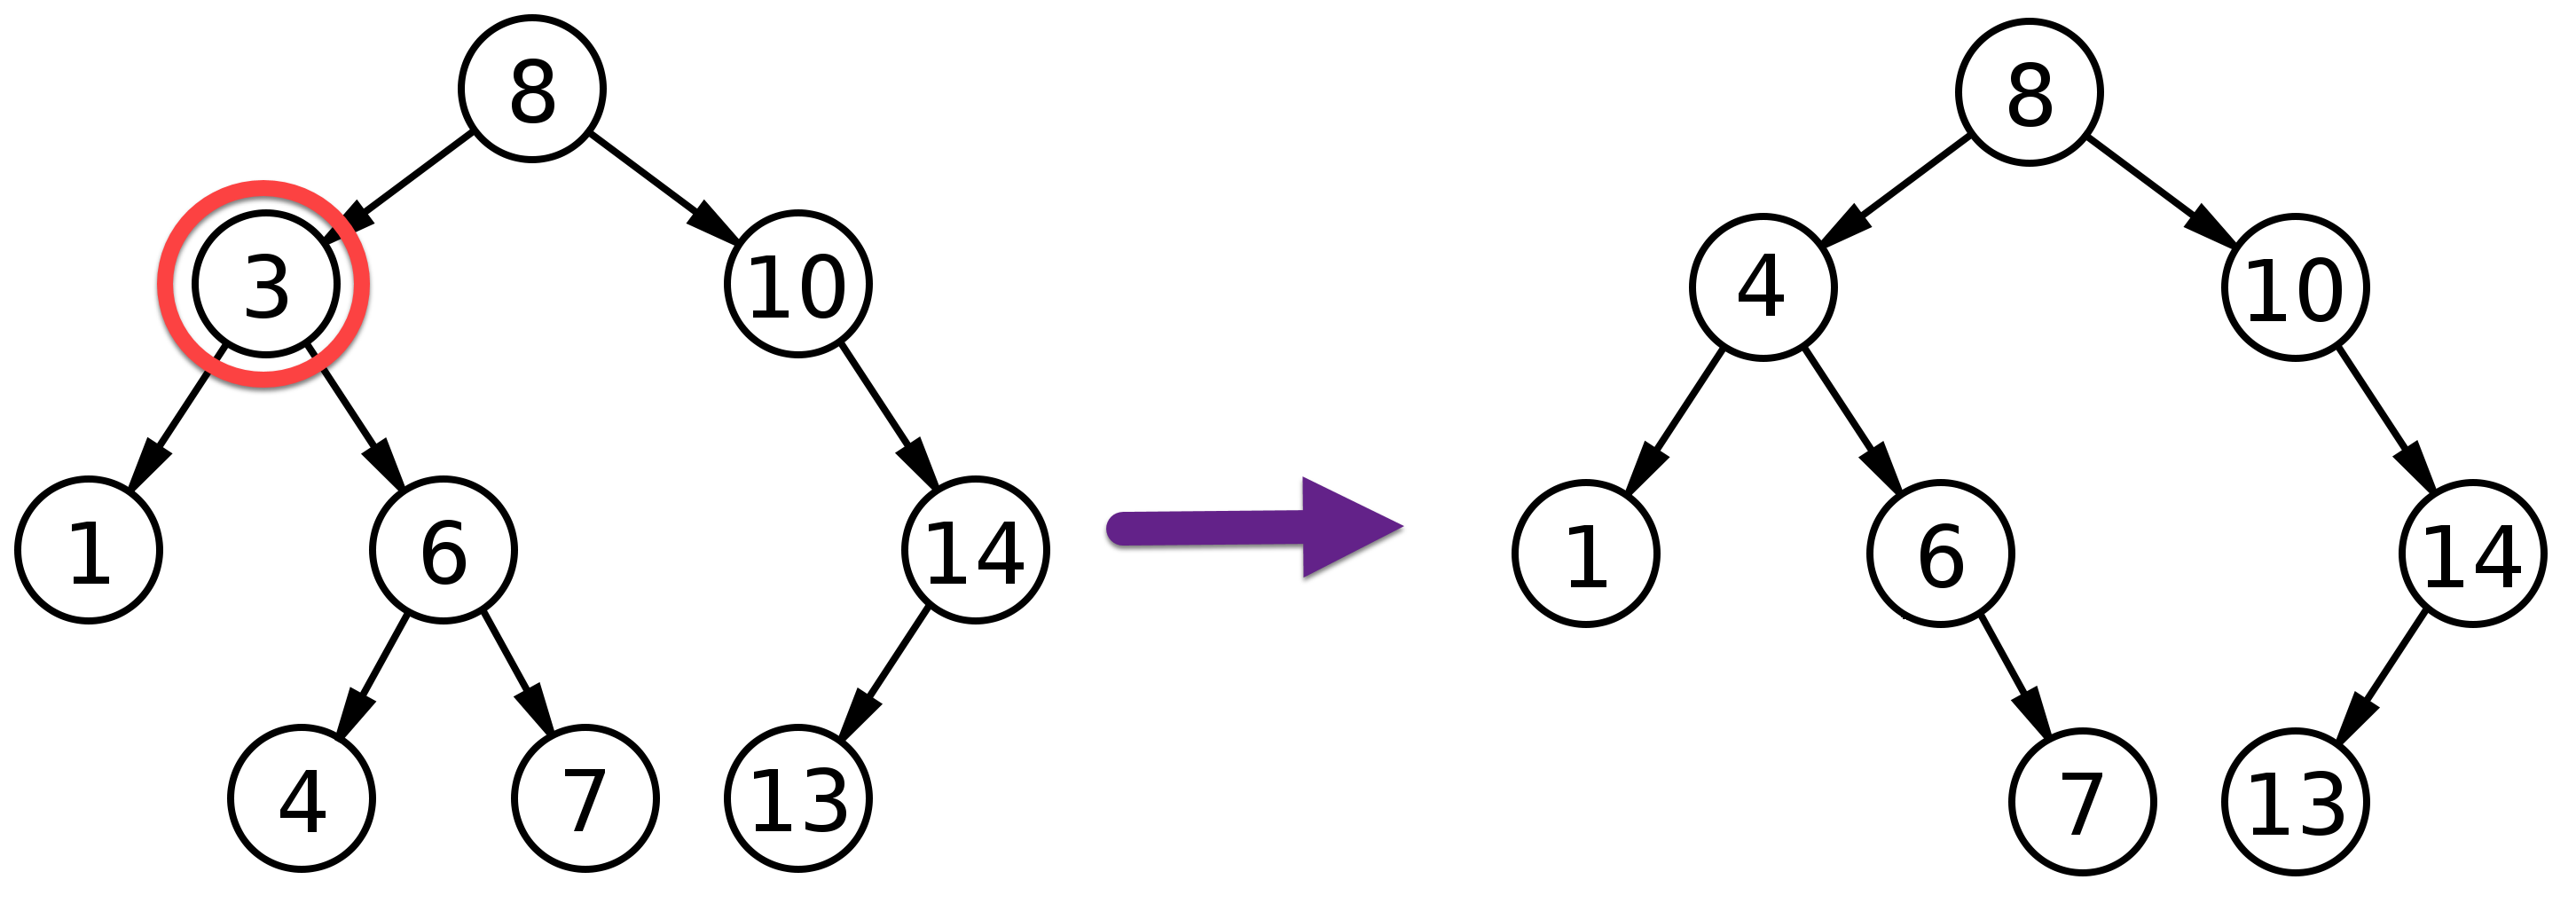
\includegraphics[scale=0.14]{img/tree4.png}
\end{frame}

\begin{frame}[fragile]
\frametitle{Binary Search Tree}
\begin{itemize}
\item Full Tree: A full binary tree is a tree in which every node other than the leaves has two children.
\item Complete Tree: A complete binary tree is a binary tree in which every level, except possibly the last, is completely filled, and all nodes are as far left as possible.
\item Perfect Tree: A pefect binary tree is a binary tree in which every level is completely filled.
\end{itemize}
\end{frame}

\begin{frame}[fragile]
\frametitle{Binary Search Tree - Sample Implementation}
{\tiny
\begin{lstlisting}
class TElement {
private:
  float data;
  TElement *left;
  TElement *right;
public:
  TElement(float data = 0.0);
  virtual ~TElement();
  void setLeft(TElement *left);
  void setRight(TElement *right);
  void setData(float data);
  TElement* getLeft();
  TElement* getRight();
  float getData();
};
\end{lstlisting}
}
\end{frame}

\begin{frame}[fragile]
\frametitle{Binary Search Tree - Sample Implementation}
{\tiny
\begin{lstlisting}
class Tree {
private:
  TElement *root;
public:
  Tree();
  Tree(const Tree & obj);
  Tree operator= (const Tree & obj);
  virtual ~Tree();
  // additional methods to use the tree
};
\end{lstlisting}
}
\end{frame}

\begin{frame}[fragile]
\frametitle{Binary Tree Traversal}
Tree traversal refers to the process of visiting each node in a tree data structure,
exactly once, in a systematic way. Such traversals are classified by the order in
which the nodes are visited.
\begin{itemize}
\item Preorder (root - left - right)
\item Inorder (left - root - right)
\item Postorder (left - right - root)
\end{itemize}
\end{frame}

\begin{frame}[fragile]
Preorder (root - left - right)\\
\vspace{1mm}
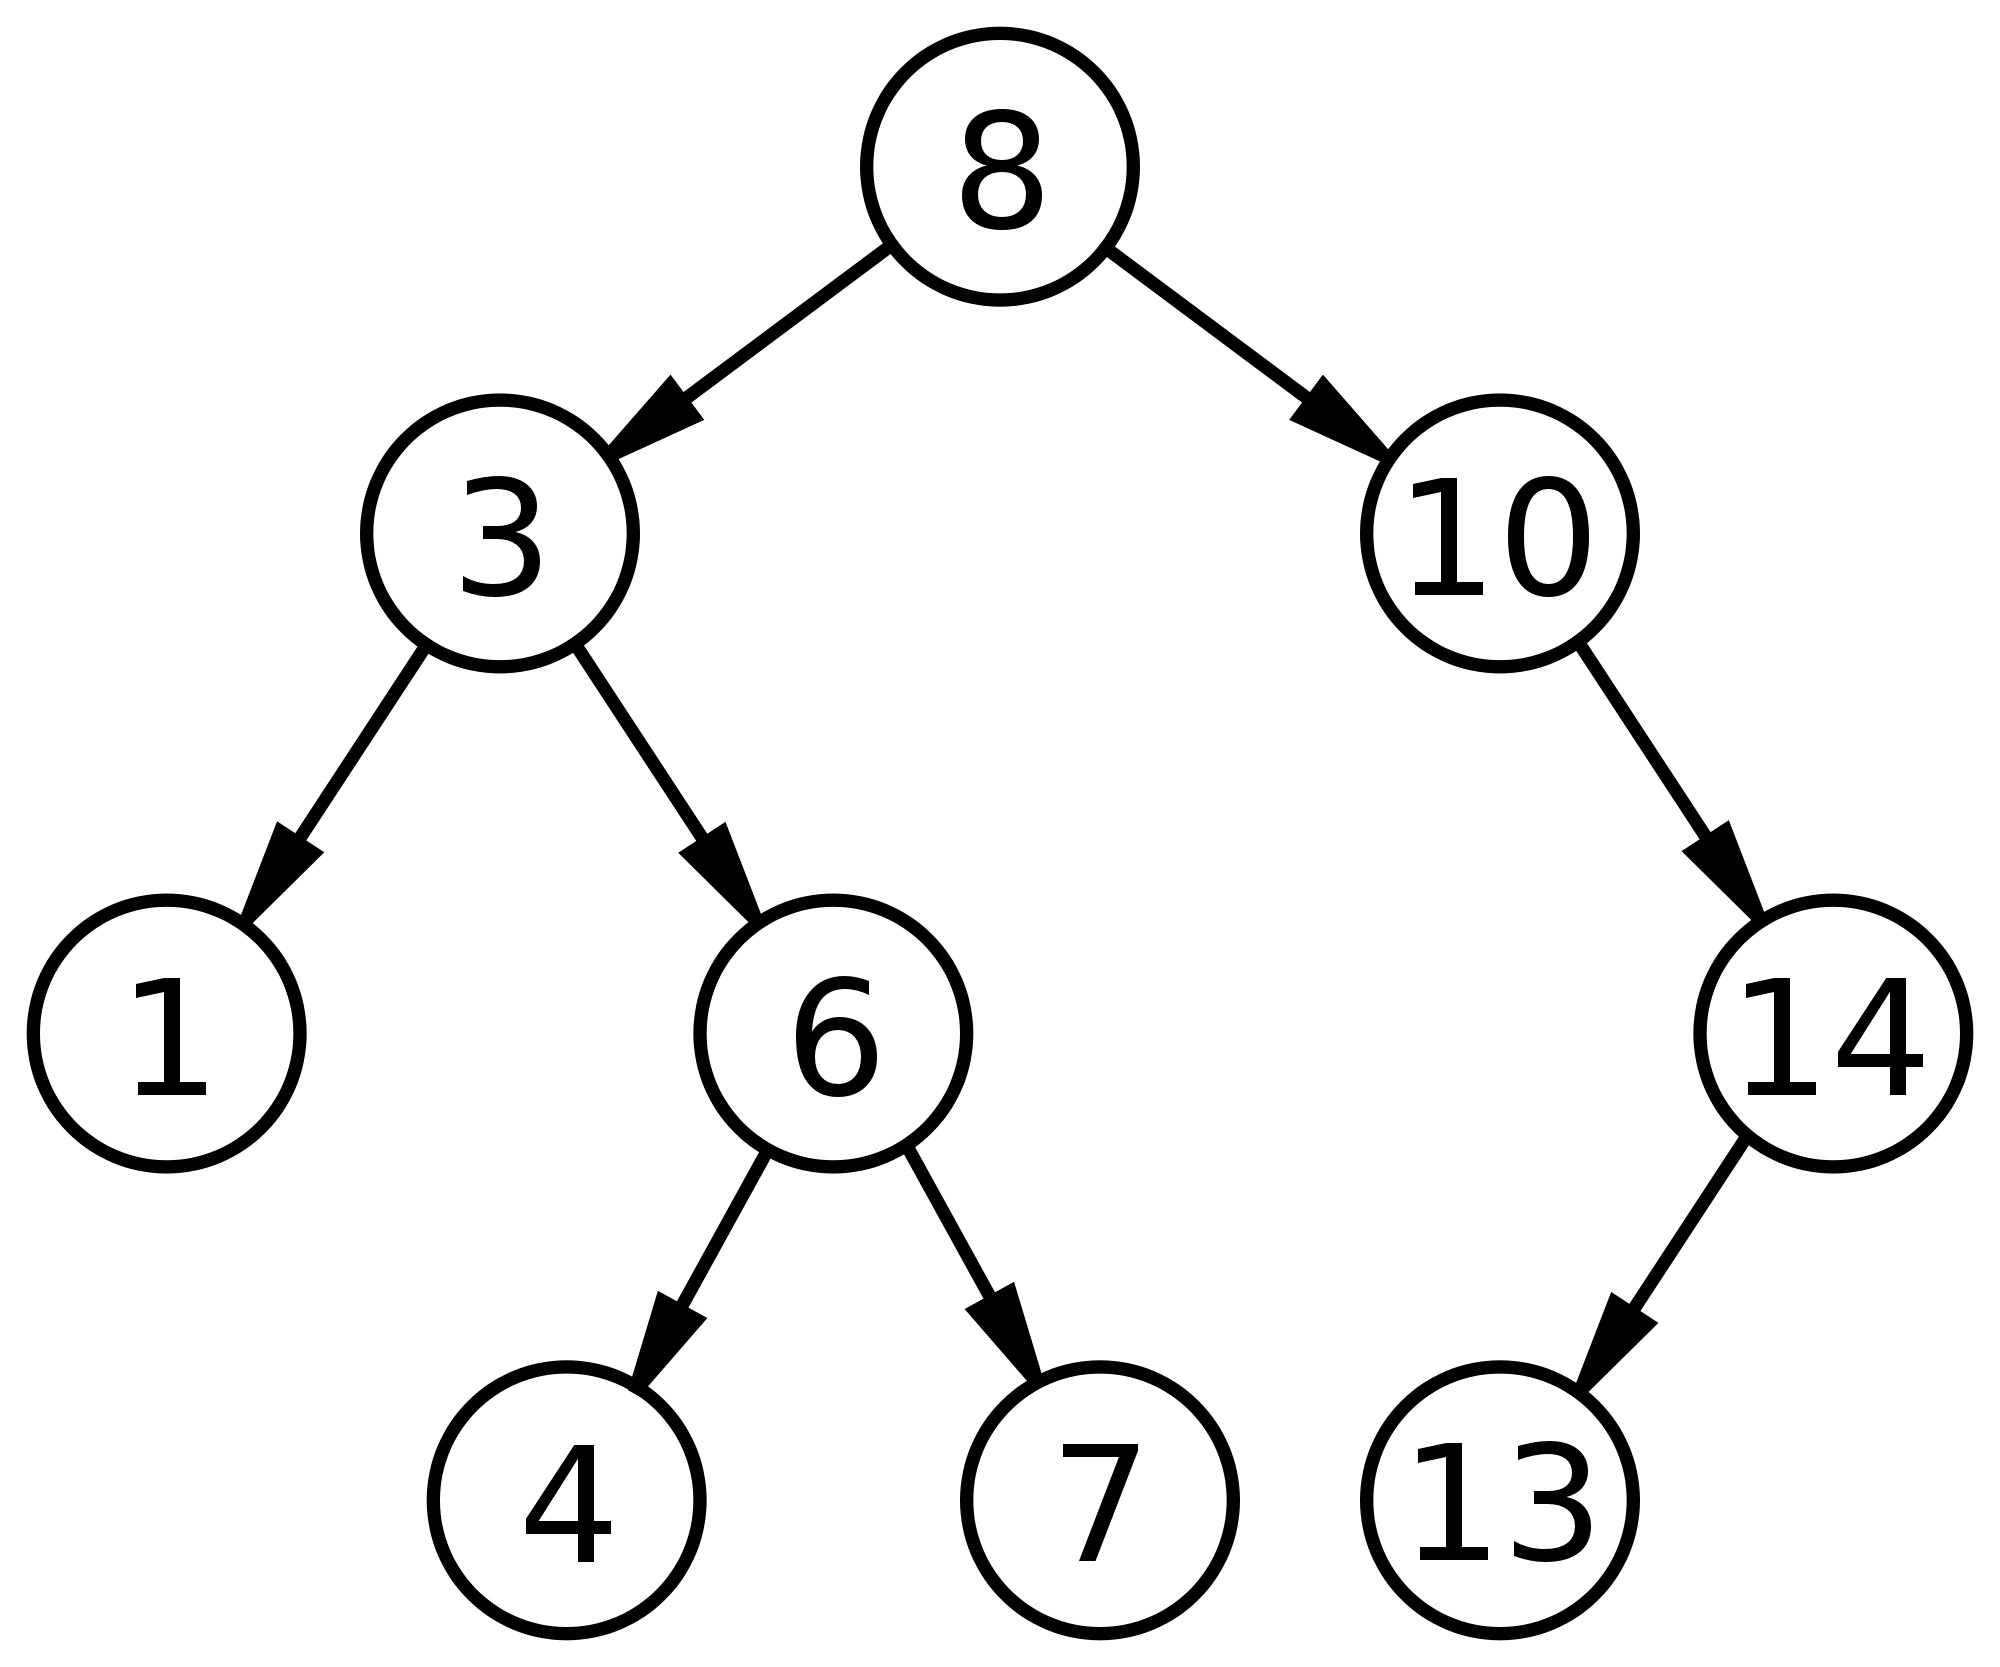
\includegraphics[scale=0.05]{img/binarytree_2.png}\\
\vspace{1mm}
8, 3, 1, 6, 4, 7, 10, 14, 13
\end{frame}

\begin{frame}[fragile]
Inorder (left - root - right)\\
\vspace{1mm}
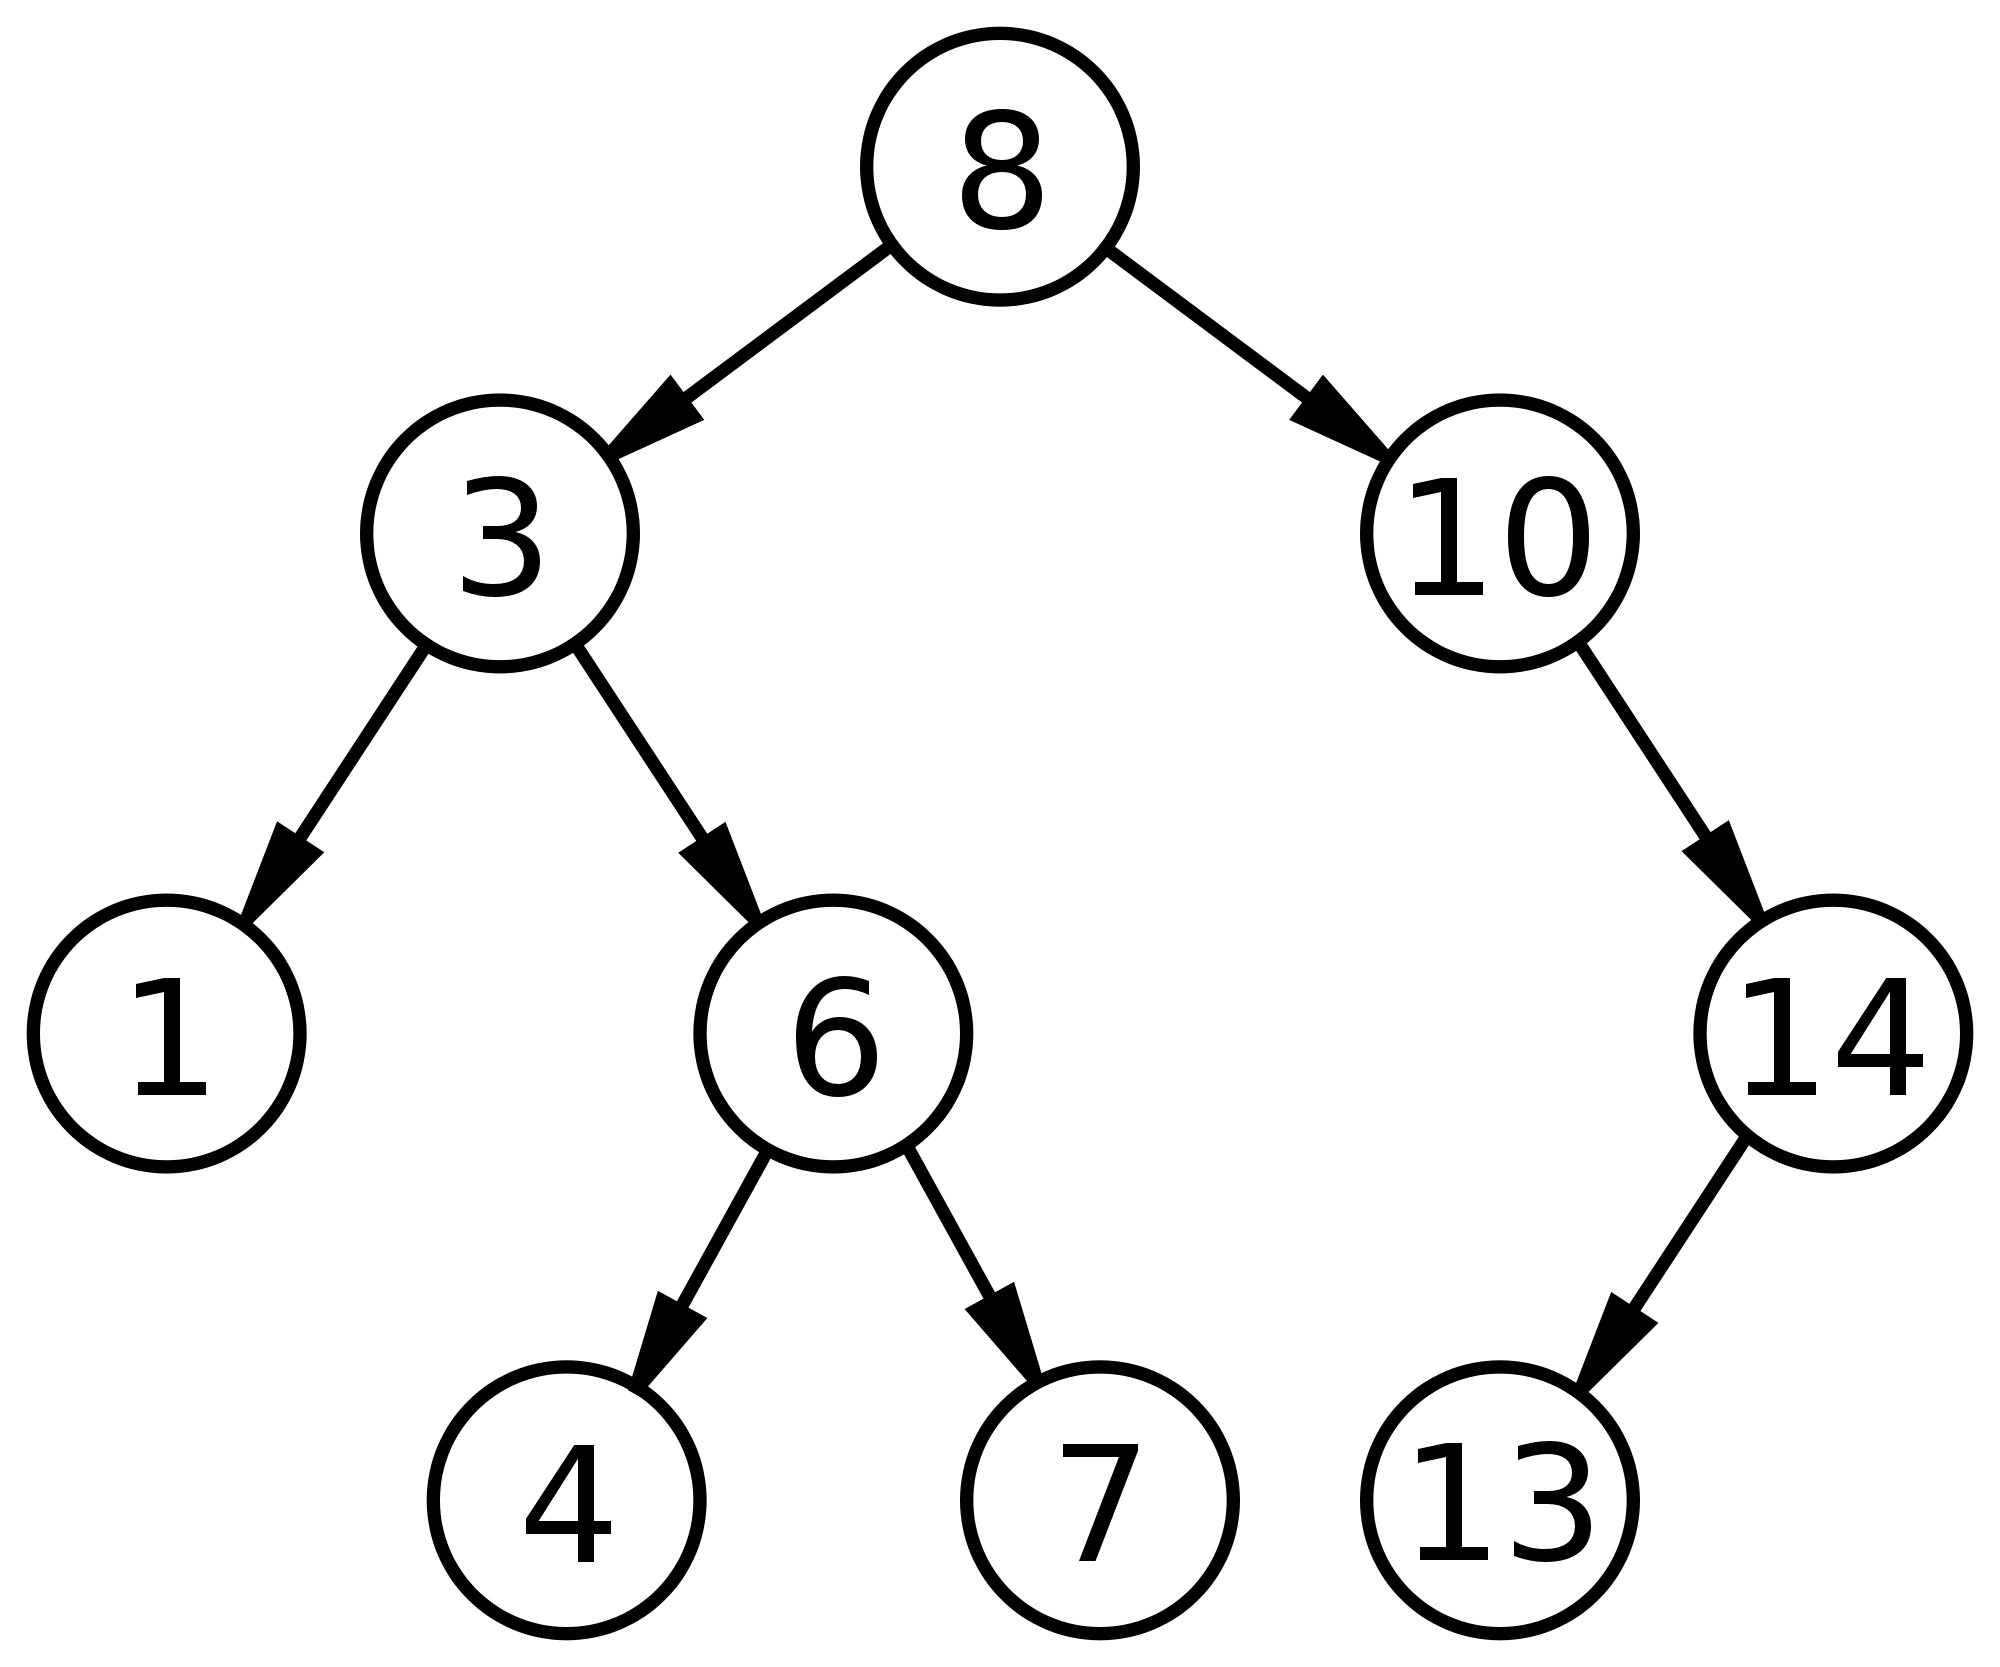
\includegraphics[scale=0.05]{img/binarytree_2.png}\\
\vspace{1mm}
1, 3, 4, 6, 7, 8, 10, 13, 14
\end{frame}

\begin{frame}[fragile]
Postorder (left - right - root)\\
\vspace{1mm}
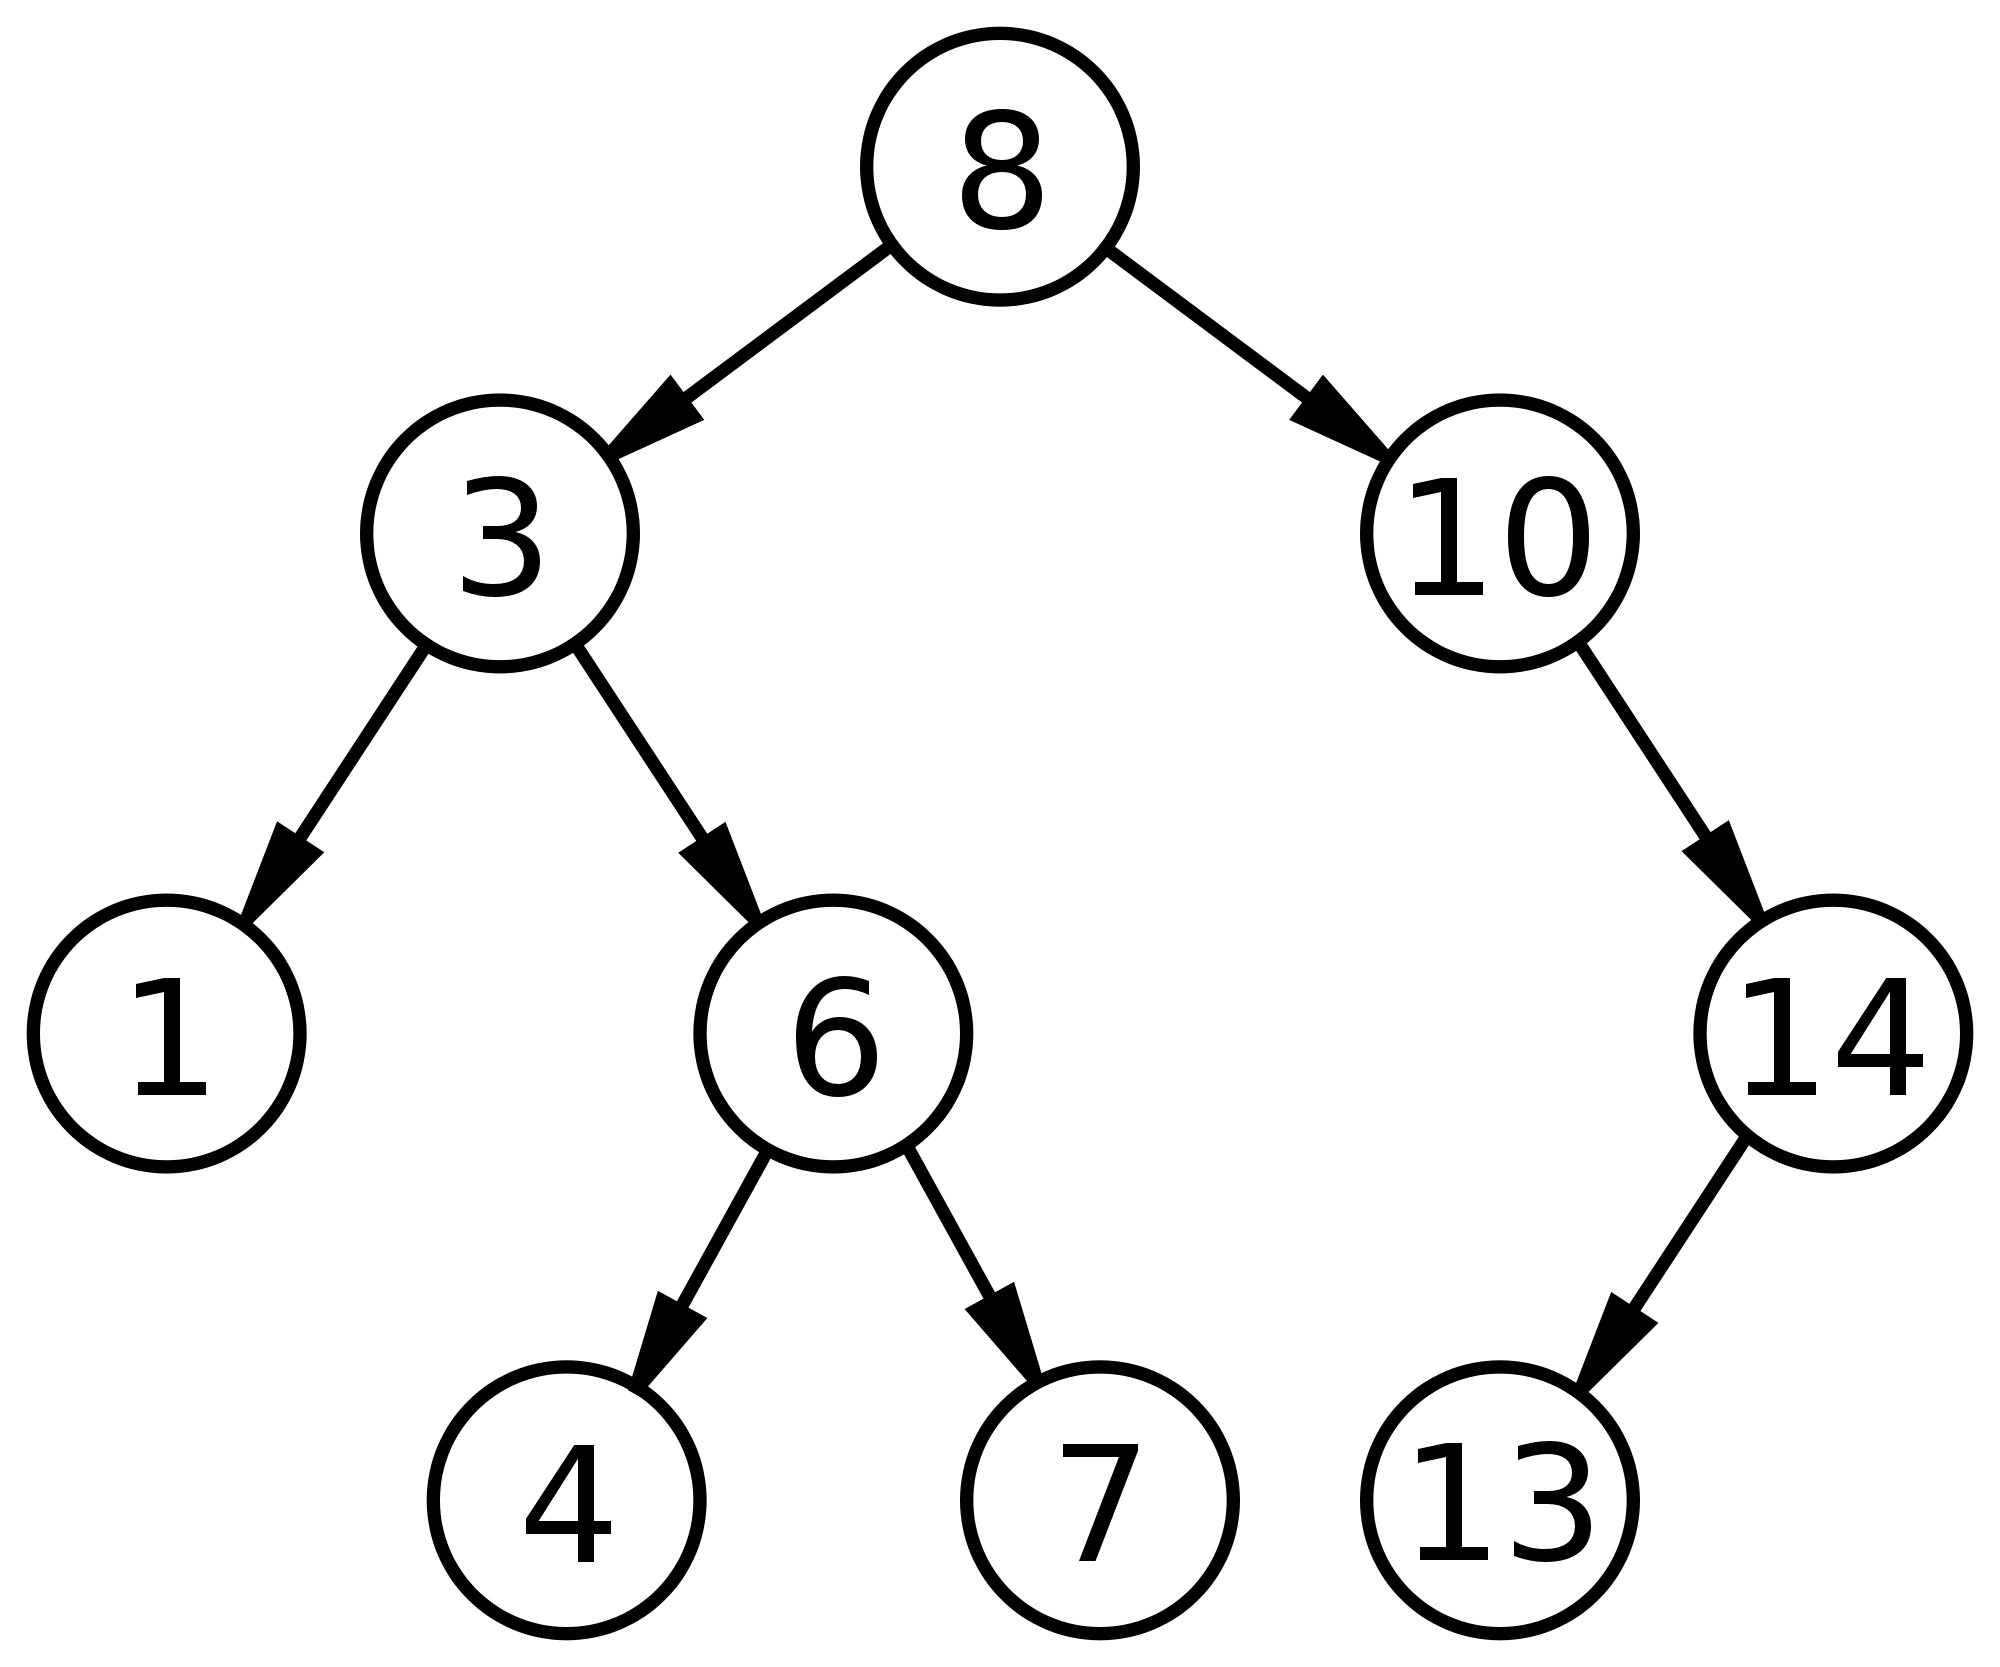
\includegraphics[scale=0.05]{img/binarytree_2.png}\\
\vspace{1mm}
1, 4, 7, 6, 3, 13, 14, 10, 8
\end{frame}

\begin{frame}[fragile]
\frametitle{Binary Tree - Exercise}
\begin{exercise}
Create a binary search tree by inserting the following elements:\\
10, 15, 5, 3, 1, 8, 13, 17, 19, 15, 9, 4\\
Delete element 10.\\
What is the order of the preorder, inorder and postorder traversal?
\end{exercise}
\end{frame}

\begin{frame}[fragile]
\frametitle{Binary Tree - Array Representation}
A binary tree could be represented with an array:
\vspace{1mm}
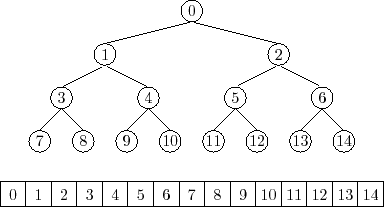
\includegraphics[scale=0.4]{img/img1156.png}\\
\vspace{1mm}
Index 0 is the root node. The children of a node with index $i$ could be calculated:
\begin{itemize}
\item $left(i) = 2i + 1$
\item $right(i) = 2i + 2$
\end{itemize}
\end{frame}

\begin{frame}[fragile]
\frametitle{Min-Heap, Max-Heap}
A heap is a specialized tree-based data structure that satisfies the heap property: if P is a parent node of C, then the key of P is less than or equal to (in a min heap) the key of C.\\
\vspace{1mm}
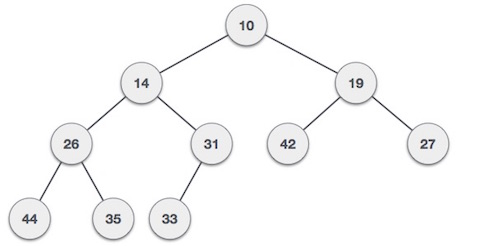
\includegraphics[scale=0.4]{img/min_heap.jpg}\\
\end{frame}

\begin{frame}[fragile]
\frametitle{Heap Operations}
Operations:
\begin{itemize}
\item extractMin (Min-Heap), extractMax (Max-Heap)
\item insert
\end{itemize}
\end{frame}

\begin{frame}[fragile]
\frametitle{Heap Operations}
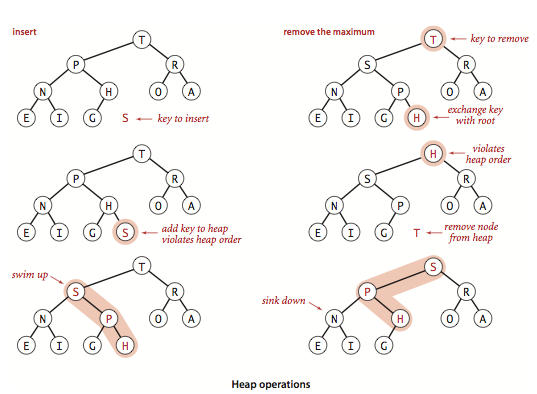
\includegraphics[scale=0.4]{img/heap-ops.png}\\
\end{frame}

